\documentclass{beamer}

\usepackage[utf8]{inputenc}
\usepackage{default}
\usepackage{graphicx}


\title{OL3-Cesium: 3D pour OpenLayers}
\author{Guillaume Beraudo}
\institute{Ingénieur Opensource \\Camptocamp, Suisse}
\date{FOSS4G\textsuperscript{fr}, 11 mai 2016}
\subject{Présentation OL3-Cesium FOSS4G-fr 2016}

\hypersetup{colorlinks,urlcolor=blue}
\setbeamertemplate{footline}[text line]{%
  \parbox{\linewidth}{\vspace*{-8pt}OL3-Cesium\hfill\insertshortauthor, FOSS4G\textsuperscript{fr} 2016}}
\setbeamertemplate{navigation symbols}{}

\begin{document}

  \begin{frame}
    \titlepage
  \end{frame}

  \begin{frame}
       \frametitle{Quoi?}
    \begin{center}
        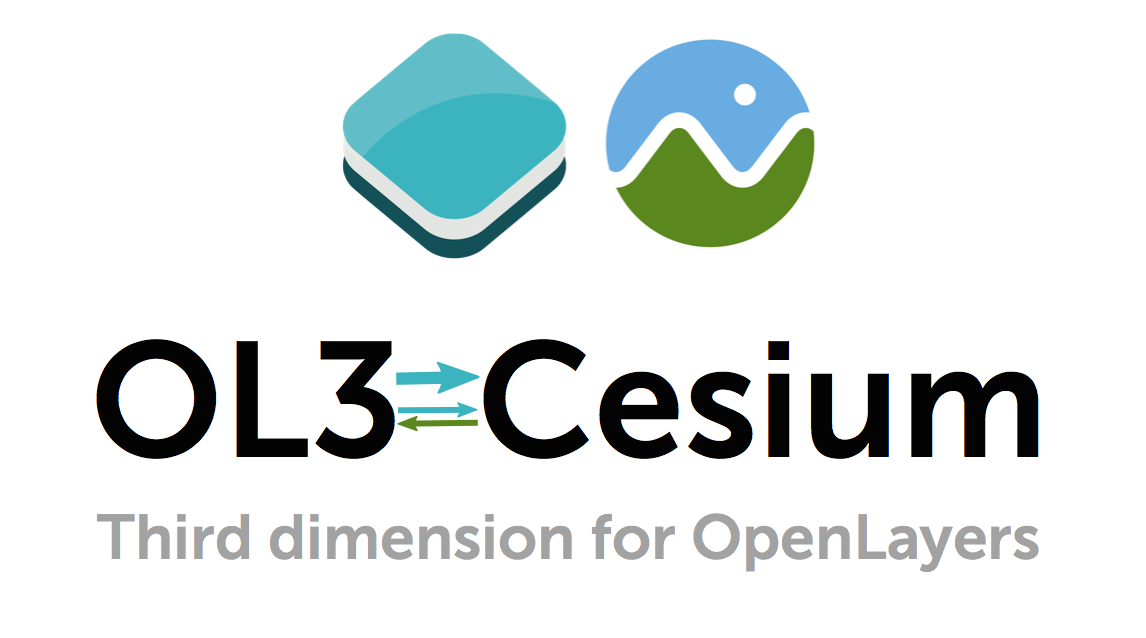
\includegraphics[width=.3\linewidth]{./ol3-cesium-wide_arrows.png}
        % ol3-cesium-wide_arrows.png: 1146x638 pixel, 72dpi, 40.43x22.51 cm, bb=0 0 1146 638
    \end{center}

      Synchronizer une carte OL3 et un globe 3D Cesium
      \begin{itemize}
      	\item Bibliothèque javascript
      	\item Licence BSD
      	\item Release stable mensuelle
      \end{itemize}
  \end{frame}


  \begin{frame}
    \frametitle{Chemin de randonnée - carte OL3}
		\begin{center}
		  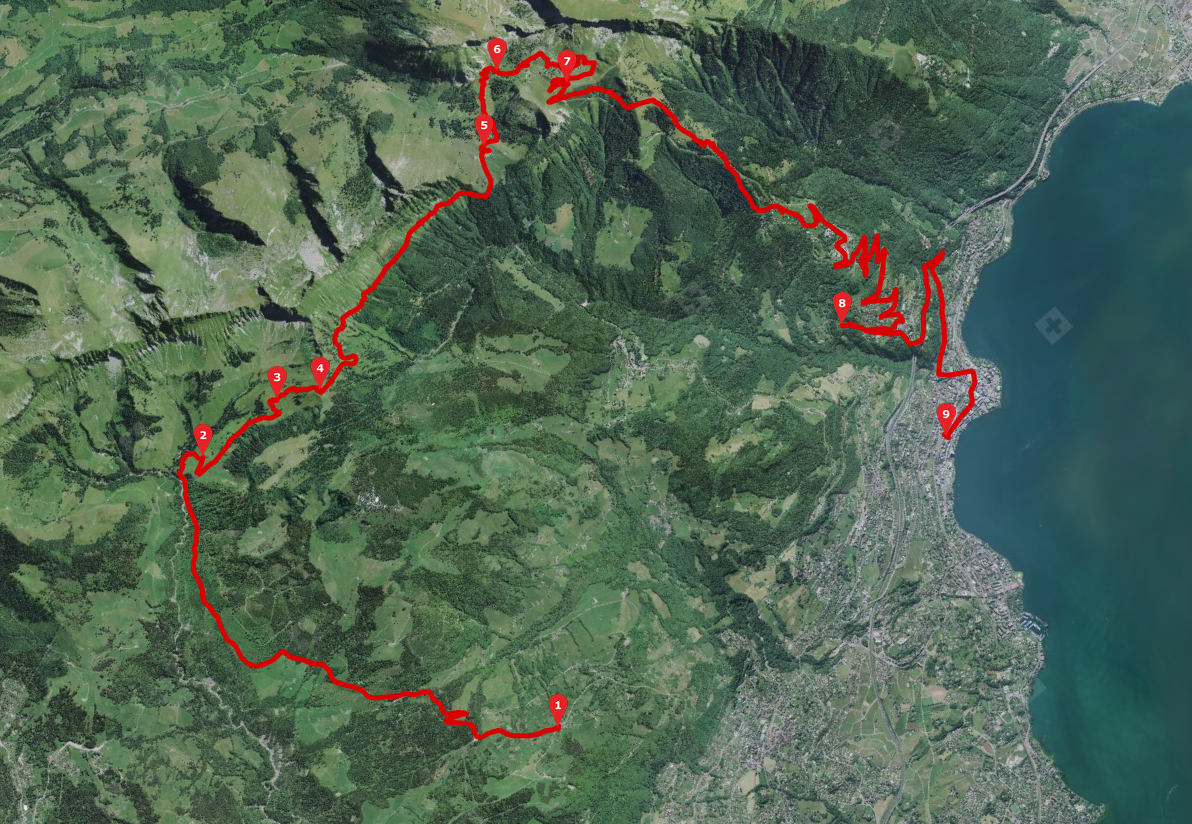
\includegraphics[width=1.0 \linewidth]{./vtt_2d.png}
		    % vtt_2d.png: 0x0 pixel, 300dpi, 0.00x0.00 cm, bb=
		\end{center}
  \end{frame}

  \begin{frame}
    \frametitle{Même chemin de randonnée - globe Cesium}
		\begin{center}
		  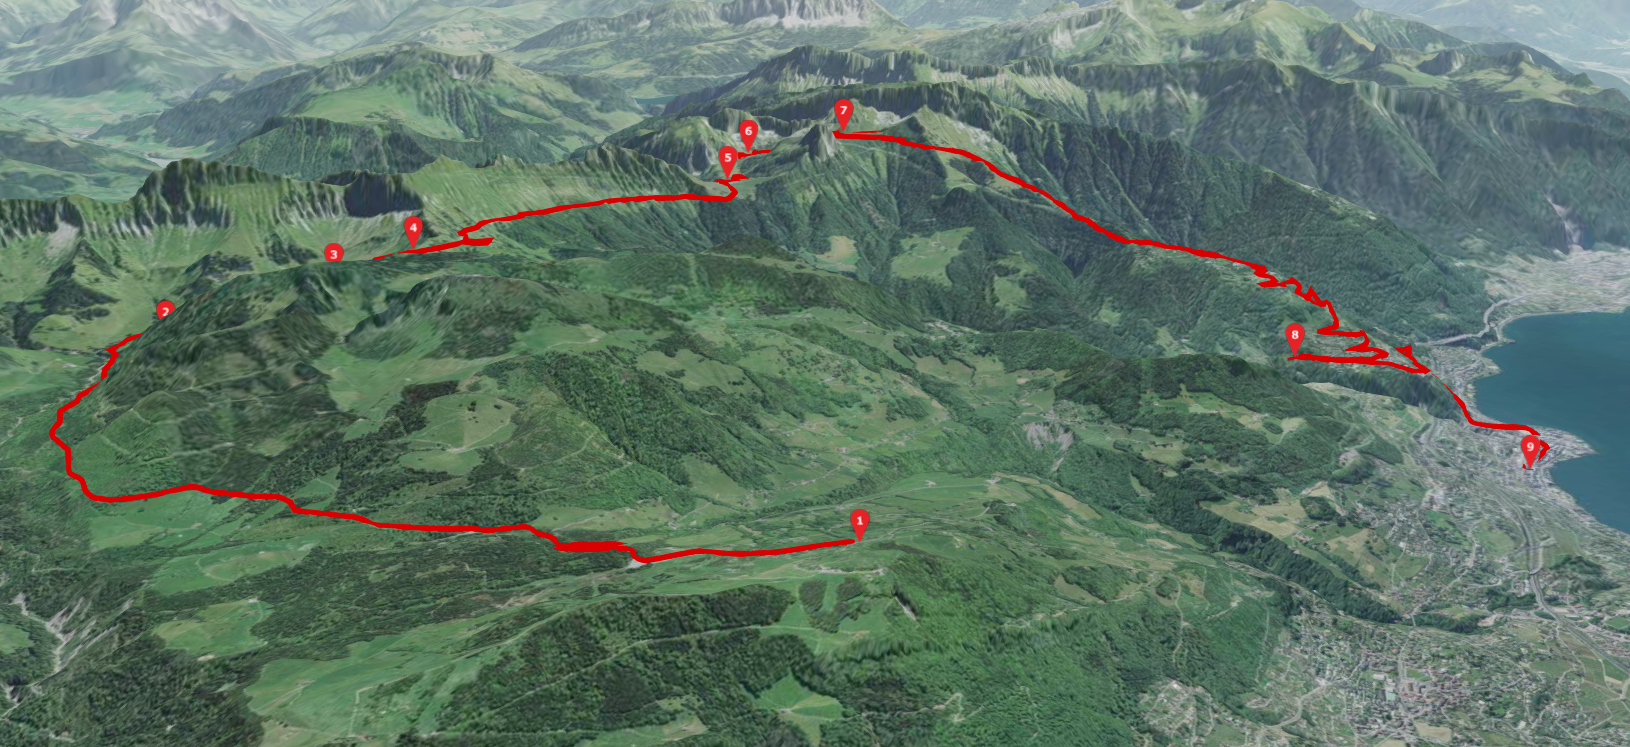
\includegraphics[width=1.0 \linewidth]{./vtt_3d2.png}
		    % vtt_3d2.png: 0x0 pixel, 300dpi, 0.00x0.00 cm, bb=
		\end{center}
    Visible en live sur \href{https://map.schweizmobil.ch/?cesium&trackId=2149217}{SuisseMobile 3D}
  \end{frame}



  \begin{frame}
    \frametitle{Pourquoi?}
	\begin{itemize}
	  \item Pourquoi Cesium?
	  \begin{itemize}
	    \item 3D
	    \item inclinaison
	    \item terrain
	  \end{itemize}
	  \pause

	  \item Pourquoi OL3?
 	  \begin{itemize}
	    \item ajusté au pixel
	    \item multi projections
	    \item léger, rapide, efficace...
	    \item API connue, déjà utilisé
	    \item utilisable sans WEBGL
	  \end{itemize}
	  \pause

	  \item Pourquoi OL3-Cesium?
 	  \begin{itemize}
	    \item évite de dupliquer la logique métier
	    \item accès aux fonctions internes d'OL3
	    \item maintenu, à jour
	  \end{itemize}
    \end{itemize}
  \end{frame}
  
  
  \begin{frame}
    \frametitle{Comment?}
    
    \begin{itemize}
      \item Automatique\newline
	    \texttt{ol3d = new olcs.OLCesium(\{map: map\})}\newline
	    \texttt{ol3d.setEnabled(true)}\newline
    \end{itemize}
    \pause
    \begin{itemize}
      \item En production\newline
      \href{https://map.geo.admin.ch/}{Géoportail de la confédération Suisse} (\href{https://github.com/geoadmin/mf-geoadmin3}{code source})
    \end{itemize}
  \end{frame}


   \begin{frame}
    \frametitle{Fonctionnement interne}
    \begin{itemize}
      \item olcs.OLCesium
        \pause
      \item olcs.AbstractSynchronizer
        \begin{itemize}
          \item olcs.RasterSynchronizer
          \item olcs.VectorSynchronizer
        \end{itemize}
        \pause
      \item olcs.FeatureConverter
    \end{itemize}
  \end{frame}


  \begin{frame}
    \frametitle{Challenges et solutions}
    \begin{itemize}
      \item Cesium vide la batterie (utiliser l'autorenderloop)
        \pause
      \item Reprojection de rasters (créer son synchronizeur)
        \pause
      \item Lignes sur le terrain (utiliser des coordonnées 3D)
        \pause
      \item Clusters raster (reprojeter ou utiliser ol3-cluster-tool)
     \end{itemize}
  \end{frame}

  \begin{frame}
    \frametitle{Clusters 3D vectoriels}
    Visible sur \href{https://map.schweizmobil.ch/?cesium&trackId=2149217&layers=Train}{SuisseMobile}
    \begin{itemize}
      \item 30'000 points au lieu de reprojeter le raster
      \item Prégénéré par \href{https://github.com/gberaudo/ol3-cluster-tool}{ol3-cluster-tool}
      \item Picking, données envoyées sur le GPU puis décimées par le shader
    \end{itemize}
  \end{frame}

  \begin{frame}
    \frametitle{Futur}
    \vspace{-20pt}\begin{center}
      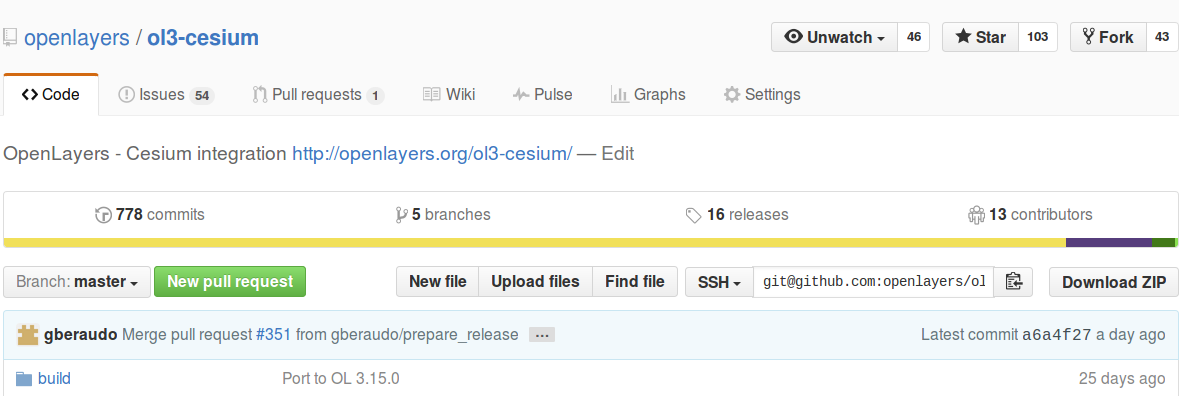
\includegraphics[width=0.9\linewidth]{./github2.png}
    \end{center}
    \begin{itemize}
      \item Continuer les releases mensuelles
        \pause
      \item Reprojection des rasters côté client?
        \pause
      \item Des idées? Vous voulez participer?
        \pause
      \item Merci, des questions?
    \end{itemize}
  \end{frame}

\end{document}
